%%%%%%%%%%%%%%%%%%%%%%%%%
% ECE539 Project Report %
%%%%%%%%%%%%%%%%%%%%%%%%%

\documentclass{article}
\usepackage{graphicx}
\usepackage{indentfirst}
\usepackage{amsmath}
\usepackage{amssymb}
\usepackage{listings}
\usepackage{url}
\usepackage{enumerate}
\usepackage{float}
\usepackage{setspace}
\usepackage{geometry}
\usepackage{siunitx}
\usepackage{pdfpages}
\usepackage{physics}
\usepackage{adjustbox}
\usepackage{hyperref}
\usepackage{fancyhdr}
\usepackage{pgffor}
\usepackage{lastpage}
\usepackage{multirow}

\geometry{letterpaper,left=2.54cm,right=2.54cm,top=2.54cm,bottom=2.54cm}
\pagestyle{fancy}
\rhead{GROUP 9}
\lhead{ECE539 PROJECT REPORT}
% \cfoot{\thepage\ of \pageref*{LastPage}}

\lstset{
  basicstyle=\ttfamily\small,
  % columns=fullflexible,
  frame=single,
  breaklines=true,
  % postbreak=\mbox{\textcolor{red}{$\hookrightarrow$}\space},
}

\title{
    ECE539 Course Project Report

    Singing Livestream Segmentation Assistant
}
\author{
    \begin{tabular}{llll}
        Group number & 9 & & \\ 
        Group members & Yushang Jin & \url{yjin248@wisc.edu} & UG \\
        & Avi Rag & \url{abalam@wisc.edu} & UG \\
        & Zalissa Kafando & \url{zongokafando@wisc.edu} & UG
    \end{tabular}
}

\begin{document}
    \setlength{\parindent}{0em}
    % \onehalfspacing
    \setlength{\parskip}{0.2\baselineskip}%
    \maketitle

    Link to our Github repo:\\
    \url{https://github.com/EricEricEricJin/ECE539-Group-Project}

    Link to our Google Drive folder:\\
    \url{https://drive.google.com/drive/folders/1L5u3G65Y_pmiLBG-jFjb8EGBnHYw5gxj?usp=drive_link}

    \paragraph*{Keywords} Audio classification, CNN, Time series, LSTM

    \paragraph*{Abstract}
    In this project we developed a program to assist cutting the singing parts out from singing livestream recordings. We used data from Bilibili, trained a CNN model that classifies each chunk of audio into speech or singing, and a LSTM model that detects the start of singing from the CNN model output. Then we developed our application method, that computes the predicted timestamps of start of singing from the LSTM output, and developed a convincing evaluation method that gives performance metrics by comparing the predicted timestamps with true labels.
    %     \tableofcontents
    \newpage

    \section{Introduction}
    Singing livestream refers to live stream singers sing in front of microphones and cameras and the pictures and audios are streamed via Internet. 
    The singers do not sing all the time, and sometimes they speak during live streaming.  

    There are always people (human) manually slicing the singing parts out from the whole live stream recordings so that other people can listen to those parts more conveniently.
    Our target is to automate this work, by \textbf{identifying the timestamps where the live streamer begins to sing}.

    Since human can quickly go over false-positive points, but missing a singing part will be bad, \textbf{we want a very high sensitivity and can sacrifice precision}.

    \paragraph*{Related works}
    A blog published by Code AI in 2021 \cite{codeai} demonstrates building a CNN model for music speech classification. They trained the model using \lstinline|gtzan| music speech dataset, and achieved 100\% validation accuracy on this dataset. The structure of the CNN in our project and part of our data preprocessing algorithms are learned from this work, but we did not copy code directly.

    % In this report, we use set $P$ to denote set of predicted markers, $Q$ to denote set of true markers, and $x$ to denote model output sequence.

    % \newpage
    \section{Data}

    We used livestream recordings on Bilibili (a video platform similar to YouTube) as raw data. By downloading and preprocessing, we obtained four datasets listed in Table \ref{dataset}.
    % \begin{table}[H]
    %     \begin{tabular}{|l|p{0.04\linewidth}|p{0.3\linewidth}|p{0.2\linewidth}|p{0.22\linewidth}|}
    %         \hline
    %         Dataset & Size & Input & Label & Source URL \\ \hline
    %         \lstinline|xxm_singing| & 274 & A person sings. Each audio 30 seconds, mono channel, 22050 sample rate & N/A & \href{https://space.bilibili.com/20159625}{Bilibili UID 20159625} \\ \hline
    %         \lstinline|xxm_speech| & 274 & A person speaks. Same format as above. & N/A & \href{https://space.bilibili.com/542262}{Bilibili UID 542262} \\ \hline
    %         \lstinline|xxm_mixed| & 10 & A person sometimes speaks and sometimes sings. Each audio about 150 minutes, mono channel, 22050Hz sample rate & \multirow{2}{1.1\linewidth}{Timestamp (h,m,s) of the beginning of each singing, crawled from bilibili description text} & \multirow{2}{1.1\linewidth}{\href{https://space.bilibili.com/1465615902}{Bilibili UID 1465615902}} \\ \cline{1-3}
    %         \lstinline|xxm_mixed_test| & 8 & Same format as \lstinline|xxm_mixed| but for testing only & & \\ \hline 
    %     \end{tabular}
    % \end{table}

    \begin{table}[h]
        \begin{tabular}{|p{0.15\linewidth}|p{0.12\linewidth}|p{0.65\linewidth}|}
            \hline
            \multirow{4}{\linewidth}{\lstinline|xxm_singing|} & Size & 274 \\ \cline{2-3}
            & Input & A person sings. Each audio 30 seconds, mono channel, 22050Hz sample rate \\ \cline{2-3}
            & Label & N/A \\ \cline{2-3}
            & Source URL & \url{https://space.bilibili.com/20159625} \\ \hline
            \multirow{4}{\linewidth}{\lstinline|xxm_speech|} & Size & 274 \\ \cline{2-3}
            & Input & A person speaks. Same format as above \\ \cline{2-3}
            & Label & N/A \\ \cline{2-3}
            & Source URL & \url{https://space.bilibili.com/542262} \\ \hline
            \multirow{4}{\linewidth}{\lstinline|xxm_mixed|} & Size & 10 \\ \cline{2-3} 
            & Input & A person sometimes speaks and sometimes sings. Each audio about 150 minutes, mono channel, 22050Hz sample rate \\ \cline{2-3}
            & Label & Timestamp (h,m,s) of the beginning of each singing, crawled from bilibili description text \\ \cline{2-3}
            & Source URL & \url{https://space.bilibili.com/1465615902} \\ \hline
            \multirow{2}{\linewidth}{\lstinline|xxm_mixed_test|} & Size & 8 \\ \cline{2-3}
            & \multicolumn{2}{l|}{Same format and type of content as \lstinline|xxm_mixed|, but for testing only}\\ \hline
        \end{tabular}
        \caption{Datasets}
        \label{dataset}
    \end{table}

    % \begin{enumerate}
    %     \item \lstinline|xxm_singing|
    %     \begin{itemize}
    %         \item Size: 274 \\
    %         \item Input: A person sings. Each audio 30 seconds, mono channel, 22050 sample rate \\
    %         \item Label: N/A \\
    %         \item URL: \url{https://space.bilibili.com/20159625}
    %     \end{itemize}
    %     \item \lstinline|xxm_speech|
    %     \item \lstinline|xxm_mixed|
    %     \item \lstinline|xxm_mixed_test|
    % \end{enumerate}

    It is strongly recommended NOT to visit source URLs directly as the website is in Chinese and its contents are not designed for academic purpose. Instead, please use our script here \url{https://github.com/EricEricEricJin/ECE539-Group-Project/tree/master/crawler} to download and preprocess the data.


    Raw inputs (videos) are downloaded from source URLs using \href{https://github.com/yutto-dev/bilili}{bilili.exe}, and converted, resampled and chunked using ffmpeg. 
    
    Labels are crawled from Bilibili video description text using selenium and parsed using regular expression. For example Listing \ref{xxm_mixed_label} is the label extracted from BV15z4y1M7ee's description text shown in Figure \ref{desc_ss}. (Please ignore the non-numerical texts. They are meaningless in our project.)

    \begin{minipage}{0.45\linewidth}
        \begin{figure}[H]
            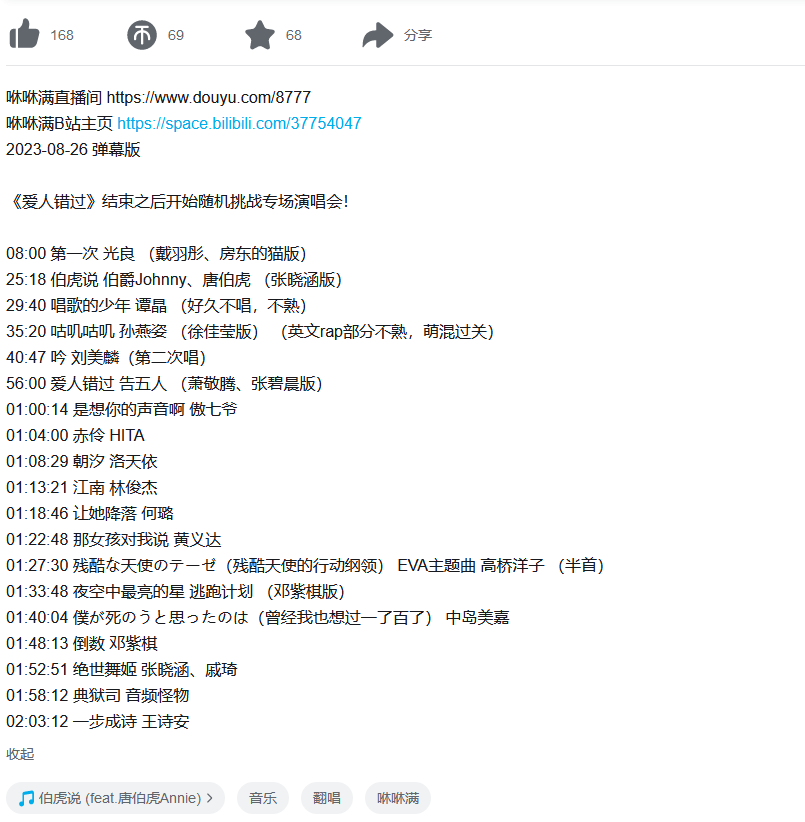
\includegraphics[width=\linewidth]{figures/desc_ss.png}
            \caption{Description text example screenshot}
            \label{desc_ss}
        \end{figure}
    \end{minipage}
    \begin{minipage}{0.52\linewidth}
        \begin{lstlisting}[
            caption={Extracted \lstinline|xxm_mixed| label example},
            label={xxm_mixed_label}
        ]
$ cat xxm_mixed/BV15z4y1M7ee.csv
0, 8, 0
0, 25, 18
0, 29, 40
0, 35, 20
0, 40, 47
0, 56, 0
1, 0, 14
1, 4, 0
1, 8, 29
1, 13, 21
1, 18, 46
1, 22, 48
1, 27, 30
1, 33, 48
1, 40, 4
1, 48, 13
1, 52, 51
1, 58, 12
2, 3, 12
        \end{lstlisting}
    \end{minipage}

    
    Listing \ref{audio_format} shows the format of audio in \lstinline|xxm_singing| or \lstinline|xxm_speech| and \lstinline|xxm_mixed| or \lstinline|xxm_mixed_test| after preprocessing, just as indicated in Table \ref{dataset}. 
\begin{lstlisting}[caption={Preprocessed data format}, label={audio_format}]
Input #0, wav, from 'xxm_singing/BV11C4y1Z7hW_10_1.wav':
  Metadata:
    encoder         : Lavf58.29.100
  Duration: 00:00:30.00, bitrate: 352 kb/s
  Stream #0:0: Audio: pcm_s16le ([1][0][0][0] / 0x0001), 22050 Hz, 1 channels, s16, 352 kb/s

Input #0, wav, from 'xxm_mixed/BV15z4y1M7ee.wav':
  Metadata:
    encoder         : Lavf58.29.100
  Duration: 02:08:46.53, bitrate: 352 kb/s
  Stream #0:0: Audio: pcm_s16le ([1][0][0][0] / 0x0001), 22050 Hz, 1 channels, s16, 352 kb/s
\end{lstlisting}

    Files \lstinline|*_BV.txt| in \url{https://github.com/EricEricEricJin/ECE539-Group-Project/tree/master/crawler} lists which Bilibili videos are used.

    Train test split is realized by using \lstinline|xxm_singing|, \lstinline|xxm_speech|, and \lstinline|xxm_mixed| for training and validation only, and using \lstinline|xxm_mixed_test| for testing only. 

    % \newpage
    \section{Tasks performed}
    \subsection{Overview of this program}
    Figure \ref{overview_bd} shows the general block diagram of our project. We developed two ML models: a CNN for classify whether a chunk of audio is singing or speech, and a LSTM to detect start of singing from sequence of probabilities output by the CNN. We used Tensorflow to implement the models.
    
    Sliding windows are applied for inference of both the CNN and the LSTM.
    \begin{figure}[H]
        \centering
        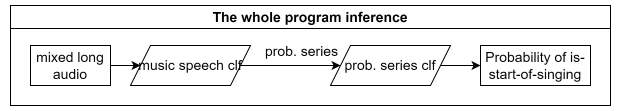
\includegraphics[width=0.8\linewidth]{figures/overview_bd.png}
        \caption{Overview block diagram}
        \label{overview_bd}
    \end{figure}

    \subsection{CNN music speech classifier}
    As shown in Figure \ref{cnn_bd}, we divide each audio file (30s) in \lstinline|xxm_singing| and \lstinline|xxm_speech| into 5 parts so that there are 6 seconds (132300 samples) each partition, and have $274 \times 5=1370$ inputs each category in total. Then we apply Fourier Transform with sliding window length=255, step=128 on audio and get spectrograms with size 1032x129. Then compress the spectrogram to size 512x64 and feed into the CNN. 

    The target is one-hot encoding of speech (0) and singing (1).
    \begin{figure}[H]
        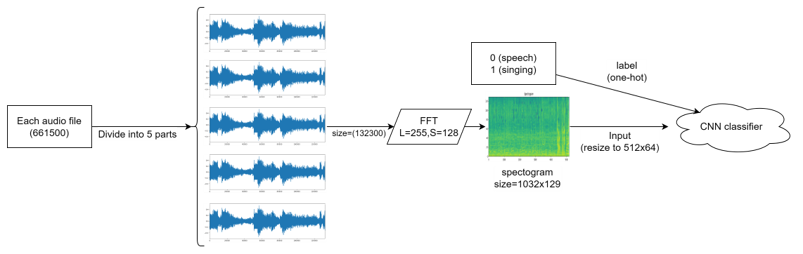
\includegraphics[width=\linewidth]{figures/cnn_bd.png}
        \caption{CNN classifier data flow}
        \label{cnn_bd}
    \end{figure}
    Figure \ref{cnn_input_data} shows a speech and a singing audios' waveforms after dividing into 5 parts and their uncompressed spectrograms. In spectrograms shown, x-axis is index (time), y-axis is frequency, and z-axis is magnitude. 
    \begin{figure}[H]
        \begin{minipage}{0.49\linewidth}
            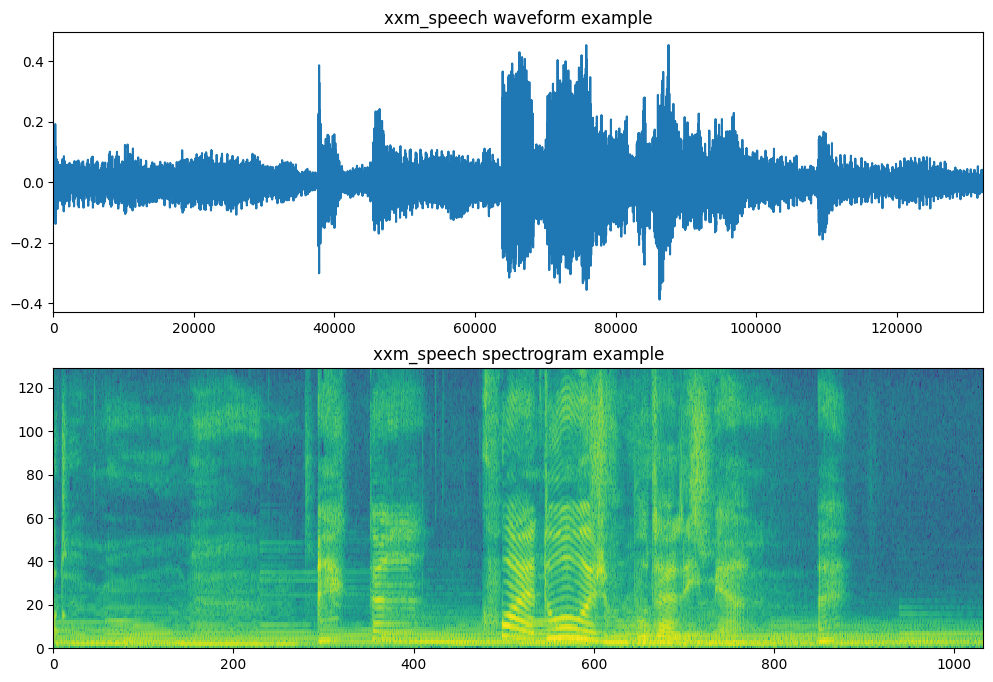
\includegraphics[width=\linewidth]{figures/spect_speech.png}
        \end{minipage}
        \begin{minipage}{0.49\linewidth}
            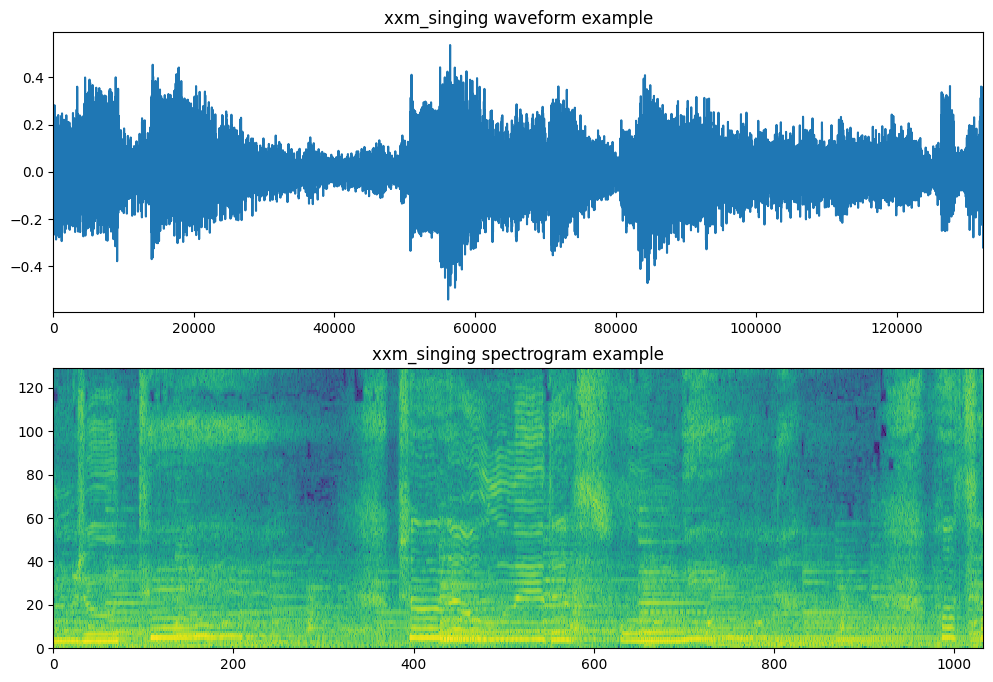
\includegraphics[width=\linewidth]{figures/spect_singing.png}
        \end{minipage}
        \caption{Example of input to CNN model}
        \label{cnn_input_data}
    \end{figure}

    The CNN model structure is shown in Listing \ref{cnn_structure}. We inherited this structure from Code AI without modifications, but we coded it in our own way.
\begin{lstlisting}[caption={CNN model structure}, label={cnn_structure}]
Model: "sequential"
_________________________________________________________________
 Layer (type)                Output Shape              Param #   
=================================================================
 resizing (Resizing)         (None, 512, 64, 1)        0         
                                                                 
 normalization (Normalizati  (None, 512, 64, 1)        3         
 on)                                                             
                                                                 
 conv2d (Conv2D)             (None, 510, 62, 32)       320       
                                                                 
 conv2d_1 (Conv2D)           (None, 508, 60, 64)       18496     
                                                                 
 max_pooling2d (MaxPooling2  (None, 254, 30, 64)       0         
 D)                                                              
                                                                 
 dropout (Dropout)           (None, 254, 30, 64)       0         
                                                                 
 flatten (Flatten)           (None, 487680)            0         
                                                                 
 dense (Dense)               (None, 128)               62423168  
                                                                 
 dropout_1 (Dropout)         (None, 128)               0         
                                                                 
 dense_1 (Dense)             (None, 2)                 258       
                                                                 
=================================================================
Total params: 62442245 (238.20 MB)
Trainable params: 62442242 (238.20 MB)
Non-trainable params: 3 (16.00 Byte)
_________________________________________________________________
\end{lstlisting}

    We applied batched training with batch size 32 and data split of 80\% for training and 20\% for validation. The optimizer is Adam and loss is binary cross entropy. Figure \ref{cnn_lc} shows the learning curve. The validation accuracy converges to 98.36\% after 11 epochs.

    Figure \ref{cnn_output} shows the example of output of inference of this trained CNN on \lstinline|xxm_mixed| with sliding window step size equals to half of chunk length, that is step = 132300 / 2 = 66150 samples = 3 seconds. Horizontal axis is time in unit second.
    \begin{figure}[H]
        \begin{minipage}{0.49\linewidth}
            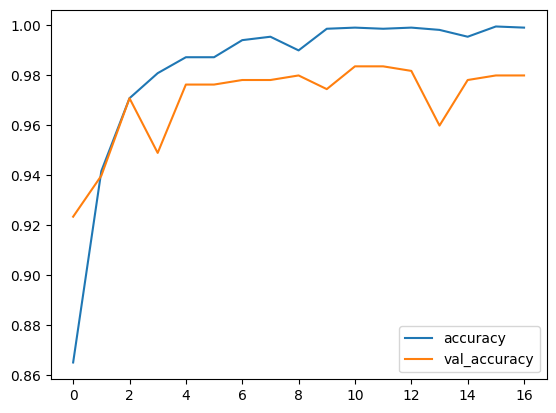
\includegraphics[width=\linewidth]{figures/cnn_lc.png}
            \caption{CNN learning curve}
            \label{cnn_lc}
        \end{minipage}
        \begin{minipage}{0.49\linewidth}
            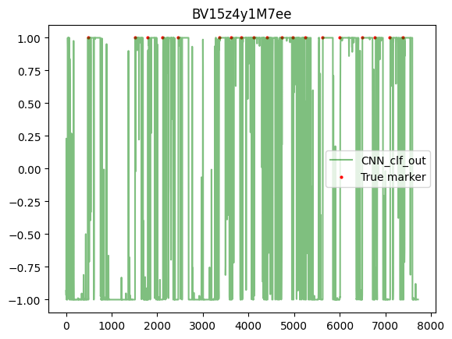
\includegraphics[width=\linewidth]{figures/cnn_output.png}
            \caption{CNN classifier output example}
            \label{cnn_output}
        \end{minipage}
    \end{figure}

    \subsection{LSTM probability series classifier}
    \paragraph*{Training data prepare}
    We extracted LSTM training input from the output of the CNN model. We inference data in \lstinline|xxm_mixed| with sliding window step size = 3 seconds (66150 samples) using the trained CNN.

    Since our target is to detect start of singing, we select 50 points of CNN output around each true marker (20 points (60 seconds) before true marker and 30 points (90 seconds) at/after true marker) as LSTM positive input, and 50 points where there is no true marker in its range as LSTM negative input. In set notation, they are defined in Equation \ref{eq_PI} and \ref{eq_NI}, 
    
    \begin{align}
        PI &= \{ [x [\frac{m}{3}-20], ..., x[\frac{m}{3}+29]]: m \in Q \} \label{eq_PI} \\
        NI &= \{ [x[i], \dots, x[i+49]]: \nexists m \in Q, i \le \frac{m}{3} \le i+49  \} \label{eq_NI}
    \end{align}
    \textit{True markers refer to the labels of \lstinline|xxm_mixed|, which are the timestamps of start of singing.\\
    Note that marker $m$ is in seconds, need to convert to index by dividing step length.}

    Figure \ref{lstm_prep_pos_input} shows example of one positive input extracted from BV15z4y1M7ee and Figure \ref{lstm_prep_neg_input} shows example of one negative input.  
    \begin{figure}[H]
        \begin{minipage}{0.49\linewidth}
            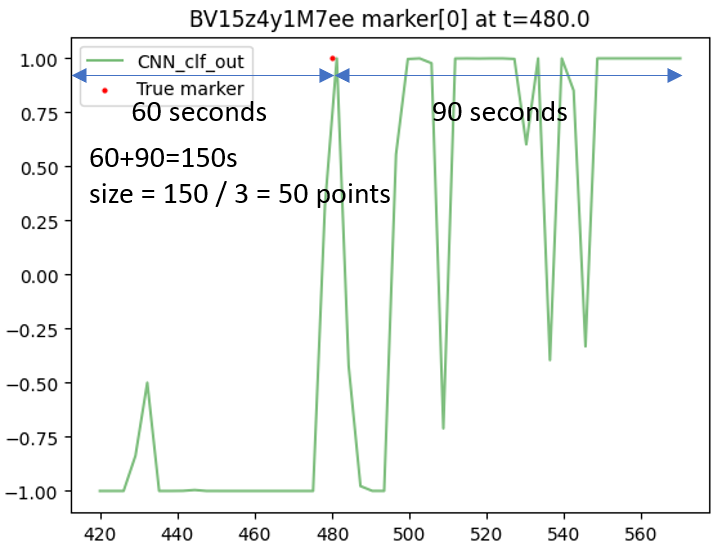
\includegraphics[width=\linewidth]{figures/lstm_prep_pos_input.png}
            \caption{LSTM positive input example}
            \label{lstm_prep_pos_input}
        \end{minipage}
        \begin{minipage}{0.49\linewidth}
            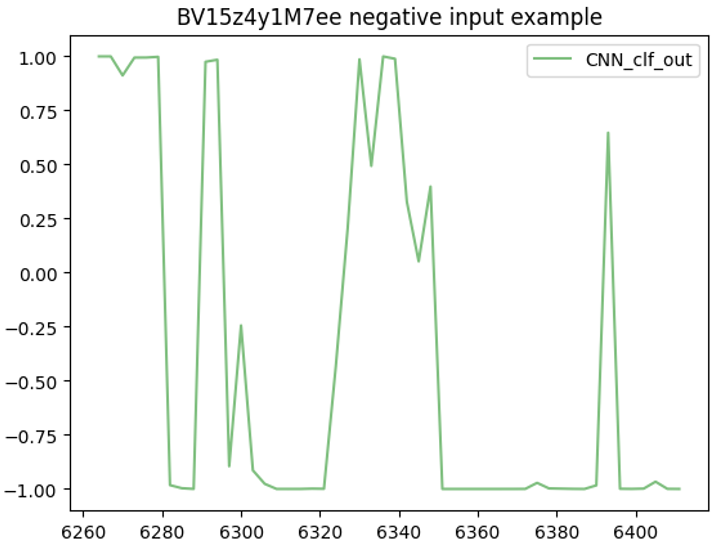
\includegraphics[width=\linewidth]{figures/lstm_prep_neg_input.png}
            \caption{LSTM negative input example}
            \label{lstm_prep_neg_input}
        \end{minipage}
    \end{figure}

    From each mixed audio we can always extract more negative inputs than positive inputs. However, to make sure each category is balanced in dataset, we  randomly choose from all negative inputs to make the number of negative inputs equals to number of positive inputs. 
    
    By this way, from each audio in \lstinline|xxm_mixed| dataset, we extracted 16 to 20 data in each category. From the 10 audios, we obtained 175 data in total for each category.

    \paragraph*{Model structure and training}
    From the way we extract input data, clearly the input size is 50.
    Listing \ref{lstm_structure} shows the structure of our single layer LSTM. We use 32 hidden units, chosen by trying a few values and 32 performs well. 
\begin{lstlisting}[caption={LSTM structure}, label={lstm_structure}]
Model: "sequential_4"
_________________________________________________________________
 Layer (type)                Output Shape              Param #   
=================================================================
 lstm_4 (LSTM)               (None, 32)                4352      
                                                                 
 dense_4 (Dense)             (None, 2)                 66        
                                                                 
=================================================================
Total params: 4418 (17.26 KB)
Trainable params: 4418 (17.26 KB)
Non-trainable params: 0 (0.00 Byte)
_________________________________________________________________
\end{lstlisting}

    We applied batched training with batch size 8 and train validation split with 80\% for training and 20\% for validation. The loss is binary cross entropy and optimizer is Adam, same to the CNN model.

    Figure \ref{lstm_lc} is the learning curve. The model converges to validation accuracy 87.14\% after 21 epochs.

    Green wave in Figure \ref{TP_FP_ex} is the output of the LSTM inference with step size = 10 points on the CNN output.

    \begin{figure}[H]
        \begin{minipage}{0.49\linewidth}
            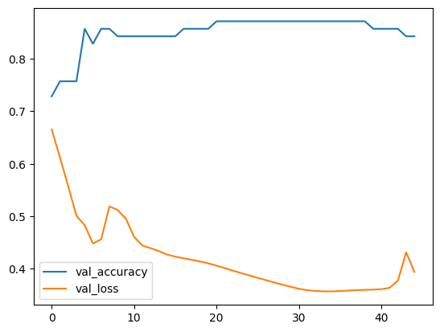
\includegraphics[width=\linewidth]{figures/lstm_lc.png}
            \caption{LSTM classifier learning curve}
            \label{lstm_lc}
        \end{minipage}
        \begin{minipage}{0.49\linewidth}
            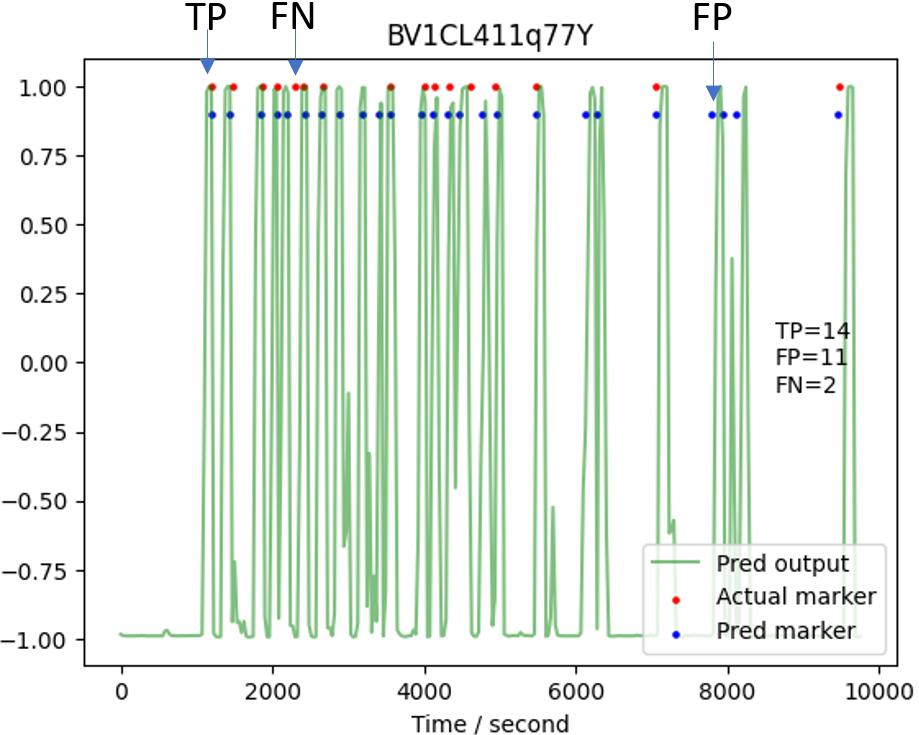
\includegraphics[width=\linewidth]{figures/TP_FP_ex.png}
            \caption{Example of LSTM output with true markers and predicted markers}
            \label{TP_FP_ex}
        \end{minipage}
    \end{figure}


    \subsection{Application and evaluation method}
    Denote the output sequence of the LSTM model above as $x$. To get the predicted time stamp of start of singing (we call predicted marker, $P$), we apply following algorithm:
    \begin{enumerate}
        \item Binarize the output
            \begin{align}
                x_b[n] = u[x[n]] = \left\{\begin{aligned}
                    0\ &\mathrm{if}\ x[n] < 0 \\
                    1\ &\mathrm{if}\ x[n] \ge 0
                \end{aligned} \right.
            \end{align}
        \item Find all continuous positive parts (ignore one-point gaps as noise) and their centers
        \begin{align}
            P &= \{ \frac{m+n}{2} \times T_0 + 60: x_b[m]=x_b[n]=1, |x_b[i]=0, i \in (m,n)| \le 1\}
        \end{align}
        $T_0 = 3 \times 10 =30$ seconds is the total step time, and add a 60-second time shift because when extracting the training inputs, start of positive input sequence is 60 seconds before the true marker. 
    \end{enumerate}

    In Figure \ref{TP_FP_ex}, predicted markers are shown in blue points.
    
    Then we compare the predicted markers $P$ with true marker $Q$ to get performance metrics
    \begin{itemize}
        \item True positives are where a true marker matches a predicted marker
        \item False positives are where a predicted marker exists but not matching any true marker 
        \item False negatives are where a true marker exists but not matching any predicted marker
        \item We do not compute true negatives here 
    \end{itemize}
    \begin{align}
        TP &= |{p \in P: \exists q \in Q, |p-q| \le L}| \\
        FP &= |P|-TP \\
        FN &= |{q \in Q: \nexists p \in P, |p-q| \le L}|
    \end{align}
    Shift threshold $L$ is the maximum time shift the user can tolerate between the predicted timestamp and the real start of singing timestamp when using our program. Here we set $L=90$, that is 1.5 minutes.

    Annotations in Figure \ref{TP_FP_ex} illustrate example of how TP, FP, FN points are counted.

    \subsection{Summary of hyper parameters engaged}
    \begin{table}[H]
        \centering
        \begin{tabular}{|p{0.16\linewidth}|p{0.5\linewidth}|p{0.26\linewidth}|}
            \hline
            Hyper parameter & Meaning & Value applied \\ \hline
            \lstinline|CHUNK_SAMPLE| & Number of sample in each chunk for classifier CNN & 661500 / 5 = 132300 \\ \hline 
            \lstinline|CLF_STEP_SIZE| & Step of slide window for using classifier to classify mixed audio & \lstinline|CHUNK_SAMPLE| / 2 = 66150 \\ \hline
            \lstinline|MLP_M| & seconds before maker included in LSTM input & 60 \\ \hline 
            \lstinline|MLP_N| & seconds at/after maker included in LSTM input & 90 \\ \hline
            \lstinline|HIDDEN_UNIT| & LSTM hidden unit number &  32 \\ \hline
            \lstinline|MLP_STEP_SIZE| & step of sliding window of using LSTM to classify predicted prob. series & \lstinline|MLP_INPUT_SIZE|/5=10 \\ \hline
        \end{tabular}
        \caption{Summary of hyper parameters}
    \end{table}
    \textit{Naming of \lstinline|MLP_M|, \lstinline|MLP_N|, \lstinline|MLP_STEP_SIZE| is due to legacy reason that we originally used MLP as post model, and did not change the variable names after moving to use LSTM. }

    % \newpage
    \section{Results and discussions}
    We applied our models, the application method, and the evaluation method on 8 audios in \lstinline|xxm_mixed_test| dataset. Figure \ref{test_wave} shows the LSTM outputs (green waves), true markers (red dots), computed predicted markers (blue dots), together with TP, FP, FN. 
    \newcommand{\addwave}[1]{
        \begin{minipage}{0.32\linewidth}
            \includegraphics[width=\linewidth]{#1}
        \end{minipage}        
    }
    \begin{figure}[H]
        \addwave{figures/test_i7dv.png}
        \addwave{figures/test_X7AP.png}
        \addwave{figures/test_t7Xb.png}

        \addwave{figures/test_J7TK.png}
        \addwave{figures/test_t7Xb.png}
        \addwave{figures/test_z7Sv.png}

        \addwave{figures/test_U7ba.png}
        \addwave{figures/test_Q7V2.png}

        \caption{Test result waveforms}
        \label{test_wave}
    \end{figure}
    
    Table \ref{test_metric} summarizes the metrics above and computes sensitivity, miss ratio, and precision.
\begin{table}[H]
    \begin{lstlisting}
BV              TP    FP    FN    Sensitivity    Miss ratio    Precision
------------  ----  ----  ----  -------------  ------------  -----------
BV1Gh4y1i7dv     9     5     0       1            0             0.642857
BV1ye411X7AP    11     1     0       1            0             0.916667
BV1n24y1t7Xb    16     6     0       1            0             0.727273
BV1os4y1J7TK    16     7     0       1            0             0.695652
BV1Hw411z7Sv    15     5     1       0.9375       0.0625        0.75
BV1JN4y1U7ba    12     3     0       1            0             0.8
BV1gu4y1Q7V2    16    18     0       1            0             0.470588
BV1CL411q77Y    14    11     2       0.875        0.125         0.56
Overall        109    56     3       0.973214     0.0267857     0.660606
    \end{lstlisting}
    \caption{Test result}
    \label{test_metric}
\end{table}

    The sensitivity is very high, for 6 out of 8 audios, they hit 100\%, and the overall sensitivity is 97.3\%. The precision is 66.1\%, which is higher than a half, meaning that the false positive points human need to go over is fewer than the true positive points. They comply with our target described in introduction that we want a very high sensitivity and precision can be sacrificed.

    % \newpage
    \begin{thebibliography}{99}
        \bibitem{codeai}
            Code AI Blogs ``Classifying Music and Speech with Machine Learning.'' Medium, \url{https://medium.com/m2mtechconnect/classifying-music-and-speech-with-machine-learning-e036ffab002e}
        \bibitem{proffdbk}
            Prof. YU HEN HU, ``Project proposal feedback'', Canvas, 10/23/2023

        \bibitem{ffmpegdoc}
            ``FFmpeg documentation'', \url{https://ffmpeg.org/documentation.html}
    \end{thebibliography}


\end{document}